\documentclass[9pt]{beamer}
\usetheme{CambridgeUS}%establece el tipo de diapositiva
\usepackage[activeacute,spanish]{babel}
\usepackage{graphicx}
\usepackage[utf8]{inputenc}

\title{Sudoku: Implementación en C++ con Qt}
\author{Iván Aveiga \\ Kevin Campuzano}
\institute{Escuela Superior Politécnica del Litoral}

\begin{document}
	\begin{frame}
		\begin{center}
			
\includegraphics[width =0.30\textwidth]{logo.png}
		\end{center}
		\titlepage
		\scriptsize
	\end{frame}

	\begin{frame}{Interfaz}{Pantalla inicial, 3puntos}
		\begin{center}
			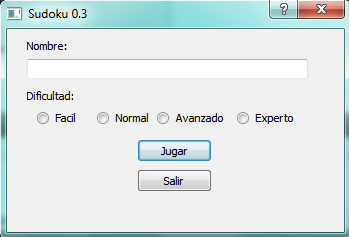
\includegraphics[width =0.70\textwidth]{inicio.png}
		\end{center}
	\end{frame}
	
	\begin{frame}{Interfaz}{Juego, generación tablero}
		\begin{center}
			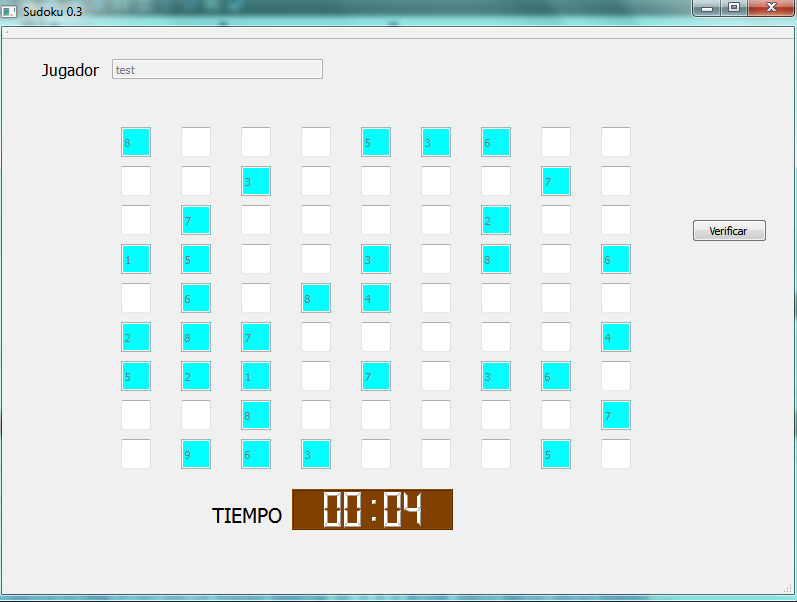
\includegraphics[width =0.60\textwidth]{juego1.png}
		\end{center}
	\end{frame}

	\begin{frame}{Interfaz}{Juego, tablero erróneo}
		\begin{center}
			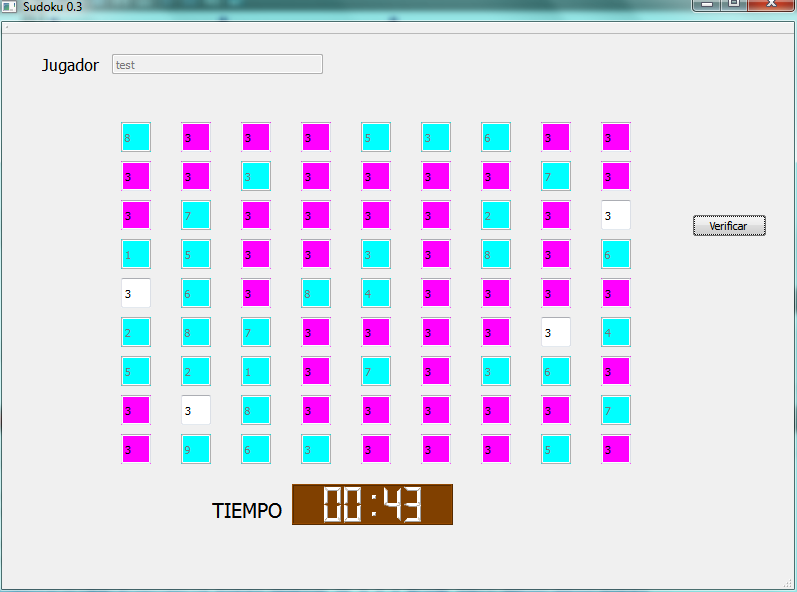
\includegraphics[width =0.60\textwidth]{juego2.png}
		\end{center}
	\end{frame}	
	
	
	

	\begin{frame}{Funcionalidad, 8 puntos}
		\begin{itemize}
			\item El tablero se genera usando el concepto de random walks sobre un sudoku ya resuelto almacenado en texto plano.
			\item El concepto de dificultad se basa en el número de celdas vacías en el tablero.
			\item Juega y Finaliza correctamente.
		\end{itemize}
	\end{frame}
	
	\begin{frame}{UML, 5 puntos}
		\begin{itemize}
			\item Diagrama de Casos de Uso
			\item Diagrama de Clases
		\end{itemize}
	\end{frame}
	\begin{frame}{UML}{Casos de Uso}
		\begin{center}
			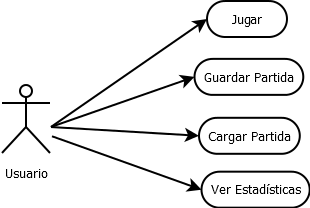
\includegraphics[width = 0.5\textwidth]{CasoDeUsos.png}
		\end{center}
	\end{frame}
	\begin{frame}{UML}{Diagrama de Clases}
		\begin{center}
			\includegraphics[width=0.7\textwidth]{clases.png}
		\end{center}
	\end{frame}
	
	\begin{frame}{Documentación}
		\begin{center}
			\includegraphics[width =0.60\textwidth]{doc.png}
		\end{center}
	\end{frame}

	\begin{frame}{Colaboración: Git, 10 puntos}{Commits por 	Integrante}
		\begin{tabular}{|c|c|}
		\hline Integrantes & # Commits \\ 
		\hline Iván Aveiga & 26 \\ 
		\hline Kevin Campuzano & 9 \\ 
		\hline Ronny Morán & 1 \\ 
		\hline 
		\end{tabular} 
	\end{frame}	
	\begin{frame}{Picos de Commits}
		\begin{center}
			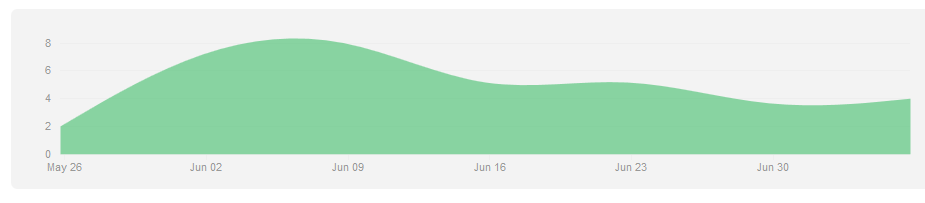
\includegraphics[width = 1.0\textwidth]{picos.png}
		\end{center}
	\end{frame}	
\end{document}